\pagestyle{n-1}
\label{n-1}

%\begin{textblock*}{5.625in}(0pt,0pt)%
%\vspace*{-3.5cm}
%\hspace*{-2.77cm}\includegraphics*[width=175.2mm]{./propagandas/N-1.pdf}
%\end{textblock*}

%\pagebreak %RIOT PUSSY
%
%\begin{center}
%
%\hspace*{.5cm}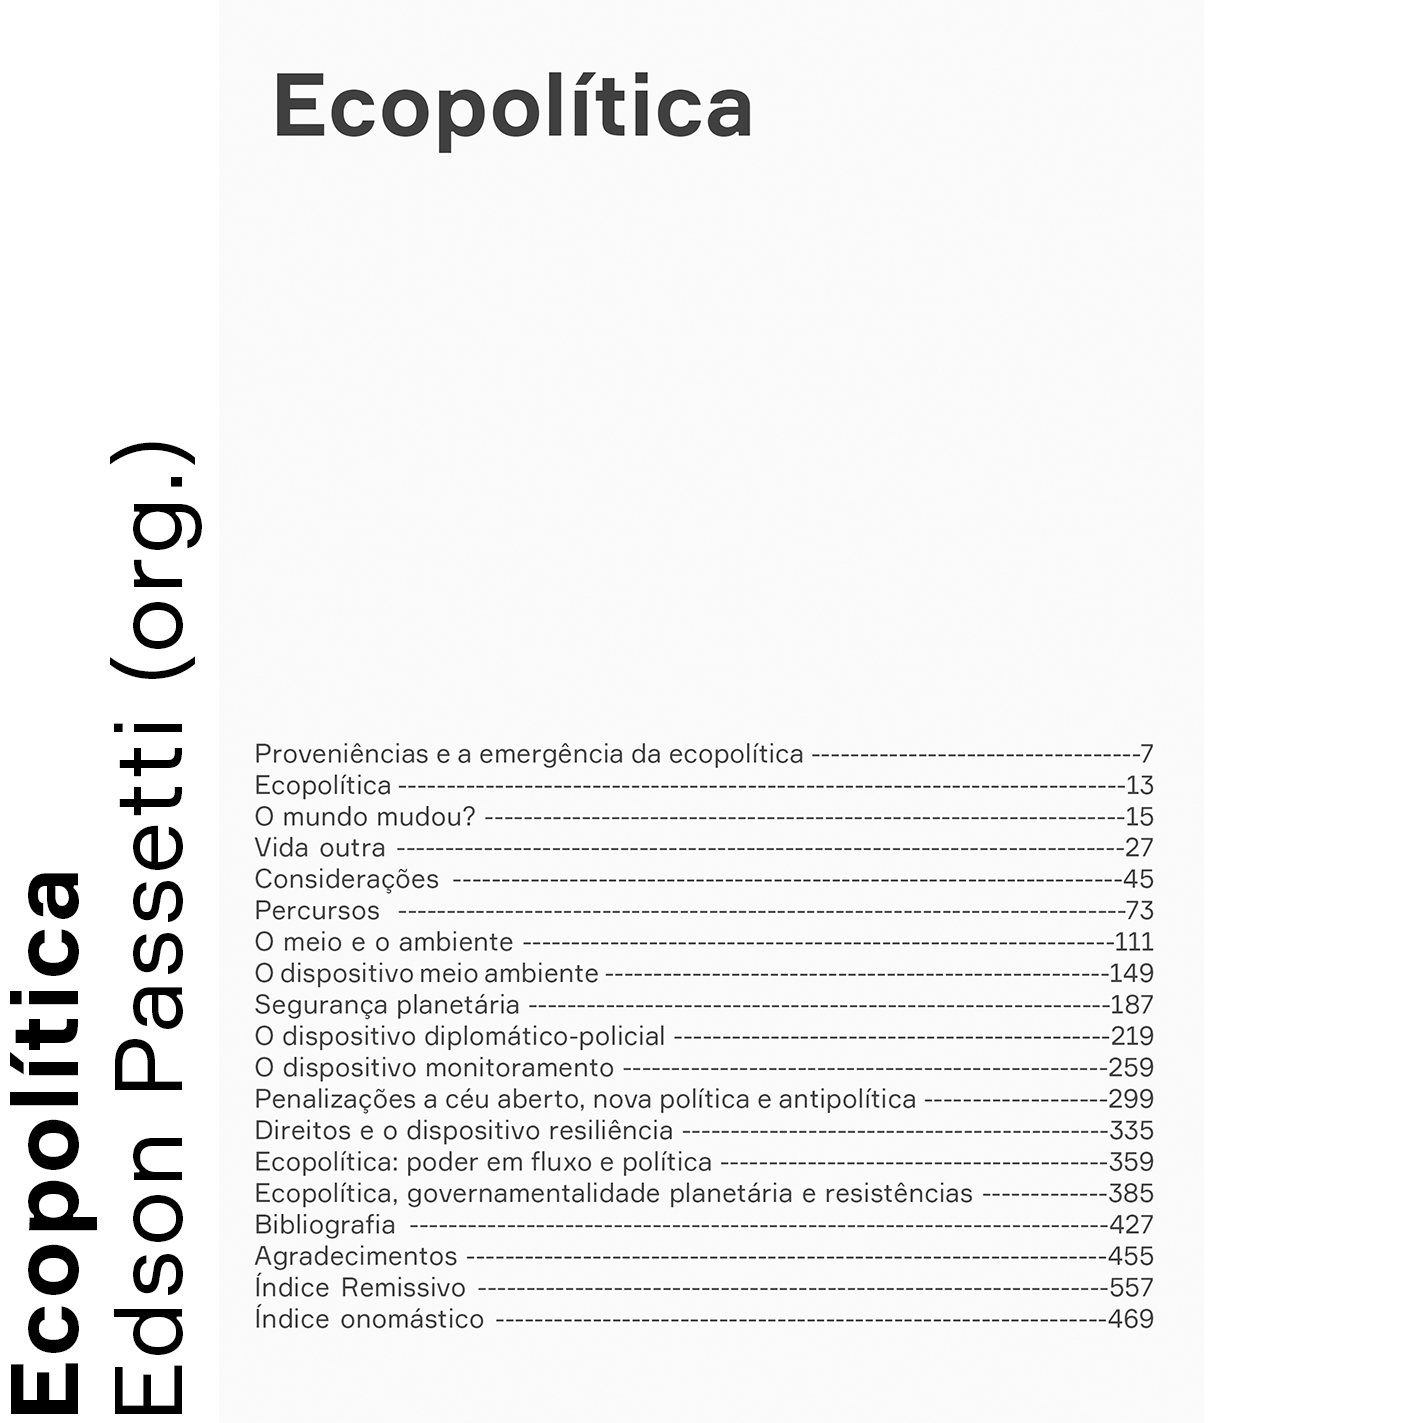
\includegraphics[width=74mm]{./grid/passetti.jpeg}
%\end{center}
%
%\hspace*{-7cm}\hrulefill\hspace*{-7cm}
%
%\medskip
%
%\noindent{}\lipsum[1]
%
%\vfill
%
%\hspace*{-.4cm}\begin{minipage}[c]{.5\linewidth}
%\small\textbf{
%\hspace*{-.1cm}Editora: n-1\\
%Título: Direito de sequência esquizoanalítica (ePub)\\
%Autor: Antoine Sibertin-Blanc\\ 
%ISBN: XXX-XX-XXXX-XXX-X\\
%%Páginas: 216\\
%%Formato: 14x21cm\\
%Preço: R\$ XX,XX\\
%}
%\end{minipage}

%\pagebreak %CORPOS QUE IMPORTAM, JUDITH BUTLER


%\begin{center}
%\hspace*{.5cm}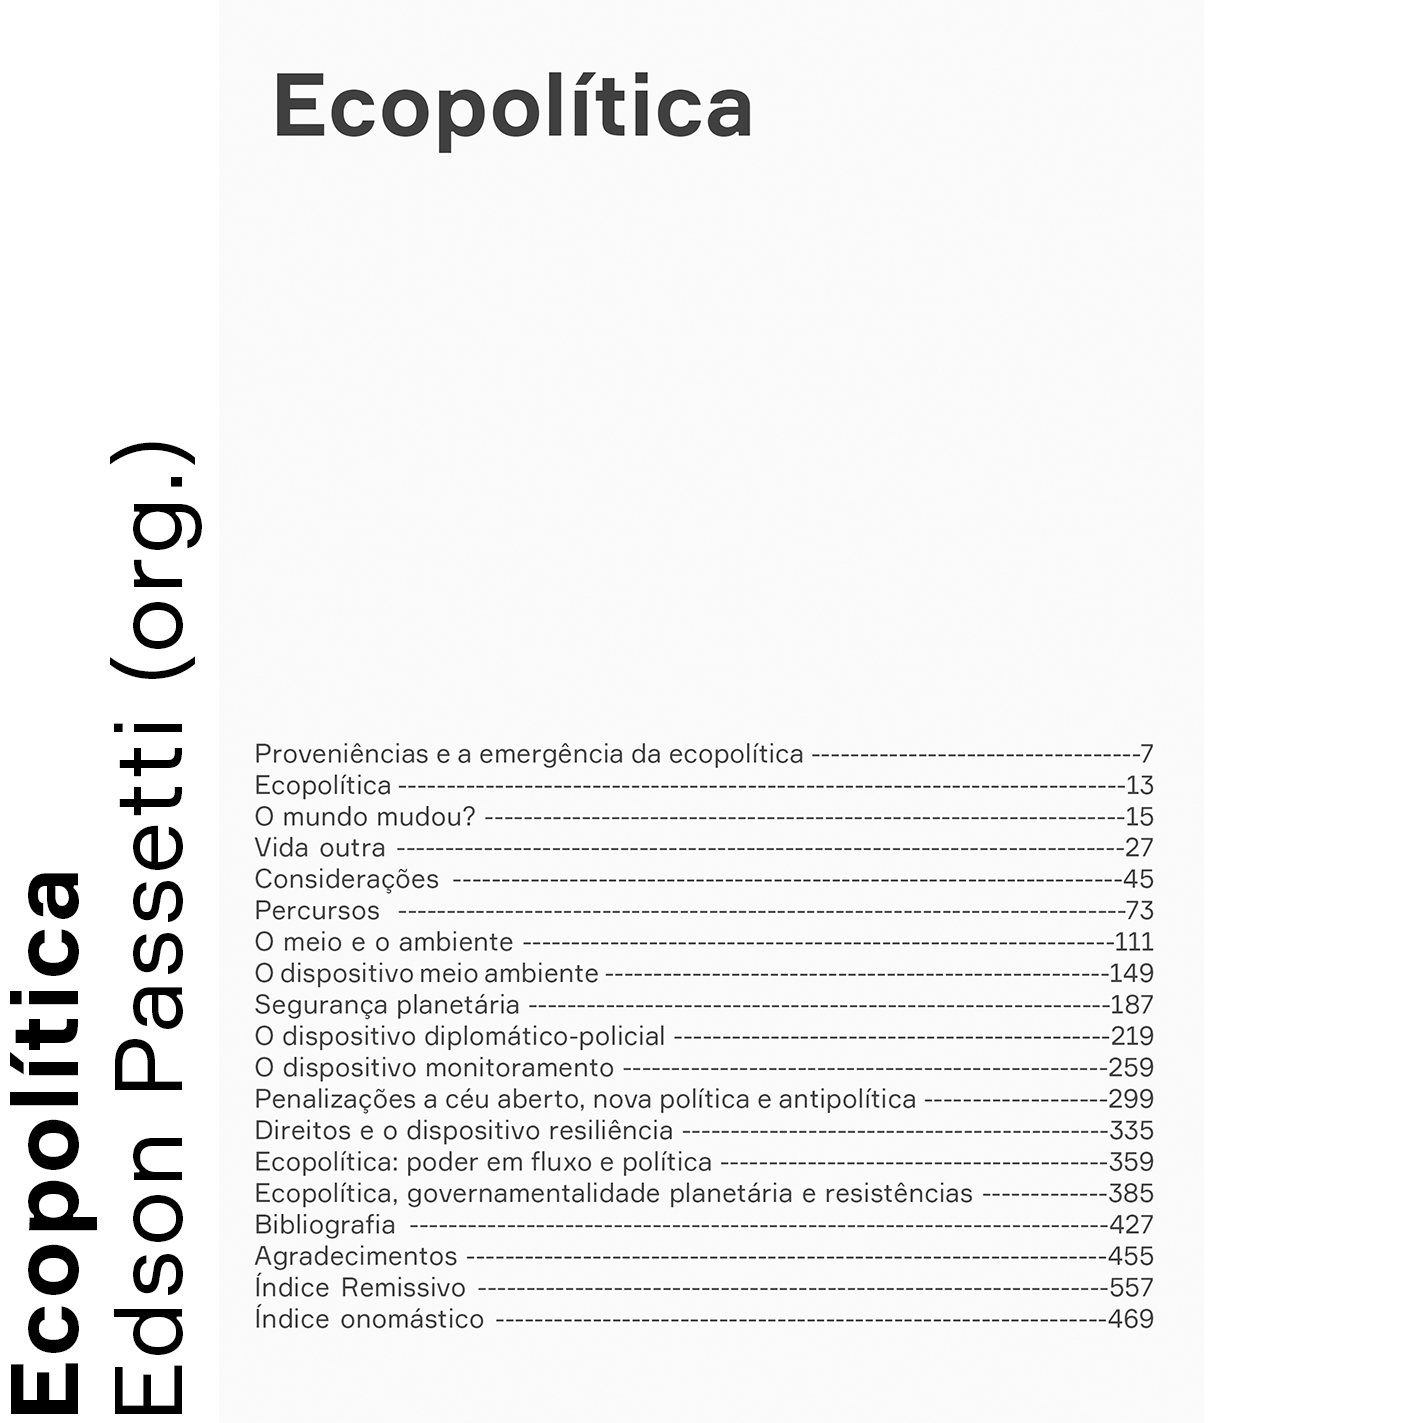
\includegraphics[width=74mm]{./grid/passetti.jpeg}
%\end{center}
%
%\hspace*{-7cm}\hrulefill\hspace*{-7cm}
%
%\medskip
%
%\noindent{}“O propósito deste livro é contribuir, a partir da África, onde vivo e
%trabalho (mas também a partir do resto do mundo, que eu nunca deixei de
%percorrer), para \hlc{uma crítica do tempo que é o nosso --- o tempo do
%repovoamento e da globalização do mundo sob a égide do militarismo e do
%capital e, como consequência derradeira, o tempo da saída da democracia}
%(ou de sua inversão). Para levar este projeto a bom termo, seguiremos
%uma abordagem transversal, atenta aos três motivos da abertura, da
%travessia e da circulação. Uma abordagem dessas só dará frutos se abrir
%espaço para uma \emph{leitura retroativa} do nosso presente.”
%
%
%\vfill
%
%\hspace*{-.4cm}\begin{minipage}[c]{1\linewidth}
%\small\textbf{
%\hspace*{-.1cm}Editora: n-1\\
%Título: Políticas da inimizade\\
%Autor: Achille Mbembe\\ 
%ISBN: 978-65-86941-17-3\\
%Páginas: 216\\
%Formato: 14x21cm\\
%Preço: R\$ XX,XX\\
%}
%\end{minipage}

\pagebreak


\begin{center}
\hspace*{.5cm}\includegraphics[width=74mm]{./grid/porno.jpg}
\end{center}

\hspace*{-7cm}\hrulefill\hspace*{-7cm}

\medskip

\noindent{}É a partir das relações entre arquitetura, tecnologia e sexualidade que \hlc{Paul Preciado aborda o império Playboy, primeira indústria de entretenimento sexual do capitalismo global}. Com um raro talento filosófico, inspirado na ideia de heterotopia de Michel Foucault, o autor inventa a noção de pornotopia, e se debruça sobre o arquipélago Playboy para entendê"-lo como realização contemporânea das utopias sexuais de Sade e tantos outros.


\vfill

\hspace*{-.4cm}\begin{minipage}[c]{1\linewidth}
\small\textbf{
\hspace*{-.1cm}Editora: n-1\\
Título: Pornotopia\\
Autor: Paul B. Preciado\\ 
ISBN: 978-65-86941-23-4\\
Páginas: 228\\
Formato: 14x21cm\\
Preço: R\$ 75,00\\
}
\end{minipage}

\pagebreak %PRAGMATISMO PULSIONAL


\begin{center}
\hspace*{-3.6cm}\raisebox{5cm}{\rotatebox[origin=t]{90}{\huge\textbf{Lançamento}}}
\hspace*{3.1cm}\includegraphics[width=74mm]{./grid/mishima.jpg}
\end{center}

\hspace*{-7cm}\hrulefill\hspace*{-7cm}

\medskip

\noindent{}O dia 25 de novembro de 1970 ficou marcado pelo seppuku do escritor Yukio Mishima no Quartel General Ichigaya de Tokyo, na presença de seus companheiros da Sociedade do Escudo --- Tatenokai. Mais do que o acontecimento em si, há uma certa concepção de corpo e de terrorismo estético que reverbera na obra deste grande escritor. \hlc{O livro \textit{Intoxicações Poéticas da Carne}, do artista brasileiro Gal Oppido, mergulha neste universo ambíguo e subversivo de Mishima criando novas imagens a partir das noções de sacrifício, homoerotismo, dor e prazer.} Há um palimpsesto de gestos que atravessam a imagem do Imperador, devaneios de Sade, o corpo sacrificado de Hijikata e tantas outras cenas que mudaram as nossas vidas.

\vfill

\hspace*{-.4cm}\begin{minipage}[c]{.8\linewidth}
\small\textbf{
\hspace*{-.1cm}Editora: n-1\\
Título: Intoxicações poéticas da carne\\
Autor: Christine Greiner e Gal Oppido\\ 
ISBN: 978-65-86941-20-3\\
Páginas: 176\\
Formato: 17,5x25cm\\
Preço: R\$ 100,00\\
}
\end{minipage}

%\pagebreak %FASCISMO OU REVOLUÇÃO? MAURICIO LAZZARATO
%
%
%\begin{center}
%\hspace*{-3.6cm}\raisebox{5cm}{\rotatebox[origin=t]{90}{\huge\textbf{Lançamento}}}
%\hspace*{3.1cm}\includegraphics[width=74mm]{./grid/mirror.jpg}
%\end{center}
%
%\hspace*{-7cm}\hrulefill\hspace*{-7cm}
%
%\medskip
%
%\noindent{}“Para além de Black Mirror” explora cinco episódios da série televisiva homônima para desenvolver complexas questões que o presente nos força a pensar. São pontos de partida para o desdobramento de reflexões urgentes: as implicações das práticas de aprovação e exclusão em uma cultura de \emph{likes}; a disseminação de linchamentos virtuais por contágios de agressividade em redes sociais, expressando"-se também na emergência de políticos explicitamente caricatos; a dificuldade de lidar com frustrações, perdas e morte, expressa, por exemplo, na promessa de paraísos hedonistas virtuais e de novos corpos sintéticos e imortais. \hlc{Entrecruzando Nietzsche, Gabriel Tarde, Henri Bergson, Deleuze e outros, esse livro embaralha os tempos e se projeta no extemporâneo, com força intempestiva frente às perplexidades que a história não cessa %de provocar.}
%
%\vfill
%
%\hspace*{-.4cm}\begin{minipage}[c]{1\linewidth}
%\small\textbf{
%\hspace*{-.1cm}Editora: n-1\\
%Título: Para além de Black Mirror: Estilhaços distópicos do presente\\
%Autor: Maria Cristina Franco Ferraz e Ericson Saint Clair\\ 
%ISBN: 978-65-86941-12-8\\
%Páginas: 180\\
%Formato: 11x18cm\\
%Preço: R\$ XX,XX\\
%}
%\end{minipage}

\pagebreak %HOMO INC.ORPORATED


\begin{center}
\hspace*{.5cm}\includegraphics[width=74mm]{./grid/homo.jpg}
\end{center}

\hspace*{-7cm}\hrulefill\hspace*{-7cm}

\medskip

\noindent{}\hlc{“Este livro é, entre outras coisas, a história de duas experiências políticas.} A primeira, que eu teria evitado e nunca teria imaginado: o inferno esquisito no qual se transformou a faculdade neoliberal \textit{à la française}, alto lugar da \textit{educastração}, da gestão do pensamento e das subjetividades, especialmente para minorias sexuais, de gênero e raciais; a segunda, o encontro com o coletivo queer e transfeminista italiano de Bolonha, o Smaschieramenti, que me transformou na hora certa.”

\vfill

\hspace*{-.4cm}\begin{minipage}[c]{.5\linewidth}
\small\textbf{
\hspace*{-.1cm}Editora: n-1\\
Título: Homo Inc.Orporated\\
Autor: Sam Bourcier\\ 
ISBN: 978-65-8694-101-2\\
Páginas: 284\\
Formato: 14x21cm\\
Preço: R\$ 65,00\\
}
\end{minipage}

\pagebreak %FERNANDO PESSOA


\begin{center}
\hspace*{-3.6cm}\raisebox{5cm}{\rotatebox[origin=t]{90}{\huge\textbf{Lançamento}}}
\hspace*{3.1cm}\includegraphics[width=74mm]{./grid/pessoa.jpg}
\end{center}

\hspace*{-7cm}\hrulefill\hspace*{-7cm}

\medskip

\noindent{}José Gil toma como matricial de todo esse processo, um alguém atenta para as mínimas sensações intersticiais que lhe sobrevêm, sensações estas tomadas como ondas transportadoras de outras sensações que se lhes associam, sensações transformadas em arte, que são também sensações de um outro, múltiplo gerador de outros. \hlc{“Escrever poemas”, diz José Gil, “é escrever segundo a lógica da heteronímia, é iniciar um processo de devir"-outro que deverá necessariamente levar à produção poética dos heterônimos''}. Sentir"-se outro, ser outro desde o primeiro ato poético da sensação, implica fazer"-se \textit{poeticamente} outros. E só existirão os heterônimos, esses outros, porque cada um deles já é outro para si mesmo, e participando todos de um vertiginoso jogo caleidoscópico. 

\vfill

\hspace*{-.4cm}\begin{minipage}[c]{.5\linewidth}
\small\textbf{
\hspace*{-.1cm}Editora: n-1\\
Título: Fernando Pessoa, ou a Metafísica das sensações\\
Autor: José Gil\\ 
ISBN: 978-65-8694-111-1\\
Páginas: 240\\
Formato: 16x23cm\\
Preço: R\$ 69,00\\
}
\end{minipage}

\pagebreak

\begin{center}
\hspace*{.5cm}\includegraphics[width=74mm]{./grid/queer.jpg}
\end{center}

\hspace*{-7cm}\hrulefill\hspace*{-7cm}

\medskip

\noindent{}Como uma rede formal (uma que, digamos, poderia ser nomeada como ré num processo judicial) \textit{Bash Back!} com certeza está morta. Como adorável terrorista tanto da direita cristã quanto da esquerda \textit{queer}, é claro que nunca existiu fora de um espetáculo. \hlc{Como uma tendência teórica, os pressupostos centrais no cerne de \textit{Bash Back!} continuam a florescer – \textit{queer negation, gender mutiny, not yr cister, baedan, filth and glitter, outlaw bodies} – muitos receptáculos e máscaras em prol de um compromisso invariável e implacável com o que é negativo e rebelde no coração da \textit{queeridade}.} Como conjunto de táticas de gangue, a \textit{Bash Back!} continua viva, sem dúvida. Mesmo quando fazemos o trabalho de antologia, nossa tarefa é incessantemente proliferada: mais viados abrindo no meio crânios de nazistas, mais \textit{queers} se rebelando simplesmente pela alegria de se rebelar, outra igreja atacada, ume jornalista desnorteade relatando sobre uma gangue \textit{queers} particularmente violenta no centrão da cidade.

\vfill

\hspace*{-.4cm}\begin{minipage}[c]{.5\linewidth}
\small\textbf{
\hspace*{-.1cm}Editora: n-1 \& Crocodilo\\
Título: Bash Back -- Ultra violência queer\\
ISBN: 978-65-86941-22-7\\
Páginas: 176\\
Formato: 12x19cm\\
Preço: R\$ 40,00\\
}
\end{minipage}

\pagebreak


\begin{center}
\hspace*{-3.6cm}\raisebox{5cm}{\rotatebox[origin=t]{90}{\huge\textbf{Lançamento}}}
\hspace*{3.1cm}\includegraphics[width=74mm]{./grid/fausto.jpg}
\end{center}

\hspace*{-7cm}\hrulefill\hspace*{-7cm}

\medskip

\noindent{}\textit{A cosmopolítica do animais} é, ao mesmo tempo, a mais importante contribuição filosófica brasileira aos \textit{animal studies} e uma obra ímpar de filosofia política. \hlc{Ao colocar a \textit{pólis}, em suas diversas configurações históricas, sob a perspectiva dos animais não humanos, Juliana Fausto abre um novo horizonte cósmico para a imaginação política}. Entretecendo com maestria fatos, histórias, experiências, conceitos e ideias hauridas das mais variadas fontes, a autora nos faz experimentar um mundo (por vir?) em que nós humanos teremos finalmente nos tornado concidadãos de nossas “espécies companheiras”.

\vfill

\hspace*{-.4cm}\begin{minipage}[c]{.5\linewidth}
\small\textbf{
\hspace*{-.1cm}Editora: n-1\\
Título: A cosmopolítica do animais\\
Autor: Juliana Fausto\\ 
ISBN: 978-65-86941-15-9\\
Páginas: 355\\
Formato: 14x21cm\\
Preço: R\$ 60,00\\
}
\end{minipage}

\pagebreak

\vspace*{1.5cm}

\noindent{}{\nohyphens{\LARGE{O que é a cosmopolítica dos animais?}}}

\bigskip

\hfill{}\scalebox{.8}{JULIANA FAUSTO}

\bigskip
\bigskip
\bigskip

\begin{multicols}{2}
\noindent{}``O homem é, por natureza, um animal político'', a célebre sentença de
Aristóteles constitui não apenas um dos fundamentos de sua teoria
política, mas um dos pilares do pensamento ocidental. Houve, e há,
defensores e detratores da ideia, mas ela é, se não inescapável,
profundamente influente. Os quatro termos da frase remetem a conceitos
complexos que suscitam disputa em relação a seu significado: homem,
natureza, animal e política. Além disso, estão conjugados de modo que
encerram questões que permanecem matéria de debate --- o homem é ou não
um animal, possui ou não uma natureza, é determinado por ela ou a
determina, a política é ou não natural, e o que quer dizer natureza ou
natural nesses contextos, entre outros pontos. Por esses e outros
problemas entrelaçados, tais como os de justiça, lei, direitos,
propriedade e formas de governo, o que se chama de filosofia política
parece ter se fixado exclusivamente no homem.

``Que o homem é um animal político em maior medida que todas as abelhas
e todos os animais de bando é claro'', continuava o filósofo grego. É
que, para ele, só o homem possuiria \emph{lógos} --- discurso, razão,
linguagem ---, o mais fundamental dos muitos avatares da distinção humana
que o pensamento ocidental produziu em sua história. Os animais, sempre
os outros diante dos quais a humanidade se eleva singularmente, além de
desprovidos de linguagem, razão, alma, ferramentas e incontáveis
propriedades, restaram sem política. \emph{Homo homini lupus}, a máxima
evocada por Thomas Hobbes, aponta para a condição

\vspace{\baselineskip}

{\small\fakereceipt{
\noindent{}“Interessam"-me, sobretudo, a situação dos animais outros que humanos e as
políticas concretas, possíveis e experimentais que os capturam, ativam,
oprimem ou são compostas com eles.”
}}

\vspace{\baselineskip}

\noindent{}bruta e bestial das
cidades em sua relação entre si, isto é, sem um Estado dos Estados que
as ordene. Sem essa autoridade superior, onde não se encontra um
mestre, retornar"-se"-ia ao estado de natureza, aquele dos lobos
considerados canibais, configuração sumamente apolítica. No debate
político, os animais surgem apenas como metáforas, símbolos --- lobos,
leões, ratos, cobras, cordeiros etc. --- que significam certas
disposições ou ânimos sem, no entanto, se referirem aos bichos e suas
populações.

Atualmente, o campo conhecido como estudos animais, que reverbera um
interesse renovado por esses outros viventes que dividem o planeta com a
humanidade, tentacularizando"-se em disciplinas de humanidades como
filosofia, literatura, antropologia, história e outras, também começa a
delinear uma teoria política animal. Volumes recentemente lançados
procuram tornar políticas questões de direito ou ética animal por meio
de sua institucionalização. O caminho seguido por este livro afasta"-se
dessa abordagem por não acreditar que política indique apenas o âmbito
das instituições políticas nas formas"-Estado. Pelo contrário, pretendo
procurar definições de política ou práticas políticas que envolvam
criativamente os animais, configurações políticas possíveis
coconstituídas.~Não desejo, com isso, abandonar o campo prático de ação,
mas investir nele em alianças cuja proeminência não seja a de
instituições humanas que, ademais, foram construídas por exclusão dos
animais. Tampouco busco a reunião ou produção de normas e diretrizes,
pois os caminhos são tão múltiplos quanto o são os modos de coabitar o
mundo pelas incontáveis populações animais (inclusive as de animais
humanos). Não se trata, portanto, de um trabalho sobre ética ou de uma
teoria política animal advinda deste, mas do deslocamento do sentido do
que se chama política. Em suma, o objetivo é traçar linhas e caminhos
que devolvam a política ao mundo e seus seres.

Interessam"-me, sobretudo, a situação dos animais outros que humanos e as
políticas concretas, possíveis e experimentais que os capturam, ativam,
oprimem ou são compostas com eles. Seja pela perda de habitat e modos de
vida, pela categorização como animais de companhia, pestes, escravos,
cobaias ou trabalhadores, nos imensos campos em que são mantidos
confinados, pela reprodução forçada, pela morte impedida e pelo
extermínio, os animais estão implicados e são atores numerosos e
potentes nas histórias e estórias que tecemos hoje, no começo do século
\textsc{xxi}, sob o signo do capitalismo liberal, na época geológica chamada
Antropoceno. É diante deles e com eles que procuro construir este texto.
Para tanto, procuro responder à exortação da filósofa ecofeminista Val
Plumwood de que devemos ser capazes de ``pensar diferentemente'', talvez
a única saída possível face à destruição atual: ``Esqueçam o modelo da
máquina passiva e nos contem mais sobre as capacidades autoinventivas e
autoelaborativas da natureza, sobre a intencionalidade do mundo não
humano.'' Se a ``mansão
das liberdades modernas repousa sobre uma base de uso de combustíveis
fósseis em permanente expansão'', e, eu acrescentaria, sobre a opressão de uma infinidade
de entes humanos e outros que humanos, e se esse movimento nos trouxe
até um momento de perigo e devastação, é preciso começar a pensar de
outro modo. Ou, antes, é preciso levar a sério a exortação de Virginia
Woolf, retomada por Donna Haraway: ``Think we must! We must
think.''

\vspace{\baselineskip}

{\small\fakereceipt{
\noindent{}“Convencida de que somente através de
encontros multiespecíficos com outros situados é possível urdir
políticas cósmicas e não exterministas, proponho um mergulho nos olhos
de alguns animais outros que humanos.”
}}

\vspace{\baselineskip}

Hannah Arendt, que inspira Haraway em seu estímulo ao pensamento --- e à
falta de pensamento que leva até a banalidade do mal ---, escreveu que
``pensar com a mentalidade alargada significa treinar a própria
imaginação a sair em visita''. Retiro propositalmente sua frase do contexto
original, profundamente ligado ao cosmopolitismo kantiano etno e
antropocêntrico, e a remeto à seguinte conclamação de Plumwood:
``Libere sua mente e faça suas próprias contribuições ao projeto de
interrupção do reducionismo e do mecanicismo. Ajude"-nos a reimaginar o
mundo em termos mais ricos que nos permitirão nos encontrar em diálogo
com e limitados pelas necessidades de outras espécies, outros tipos de
mentes. Não lhes direi como fazê"-lo. Há muitos modos de fazê"-lo. Mas
espero que os tenha convencido de que este não é um projeto diletante.
\emph{A luta para pensar diferentemente, para refazer nossa cultura
reducionista, é um projeto básico de sobrevivência em nosso presente
contexto}. Espero que vocês se juntem a ele''.

Não tenho nenhuma ilusão quanto ao que posso fazer aqui, algo
infinitamente mais modesto do que pedia Plumwood. Gostaria de pensar,
entretanto, que o espírito destas páginas vem pelo menos tangenciar essa
enorme tarefa.~Para tanto, visito algumas situações conceituais e
experimento modos de relação nos quais os animais outros que humanos
tenham a oportunidade de, existindo politicamente, ajudar a pensar de
modo diferente e a efetivamente cultivar em conjunto, para usar a
expressão de Anna Tsing, ``artes de viver em um mundo danificado''. Como
princípio, procuro sempre me referir a questões situadas, com animais
humanos e outros que humanos determinados, sejam eles povos, indivíduos
ou personagens, seguindo a indicação de Haraway que, inspirada por
Marilyn Strathern, afirma que: 
``Importa quais histórias contamos para contar histórias; importa quais
nós atam nós, quais pensamentos pensam pensamentos, quais descrições
descrevem descrições, quais vínculos vinculam vínculos. Importa quais
histórias fazem mundos, quais mundos fazem histórias''.

Pretendo, assim, escapar àquilo que Jacques Derrida chamou de o
filosofema, o discurso que toma abstratamente os animais outros que
humanos como uma imensa categoria de seres indistintos e que não se
permite ser visto por eles, entrar em relação com eles. Pensar de modo
diferente não pode supor a elaboração do animal como ``um
\emph{teorema}, uma coisa vista mas que não vê''.

Para tanto, privilegiarei algumas configurações concretas da vida dos
animais no Antropoceno, como sua existência em cidades nas feições de
\emph{pets} e errantes, o confinamento ao qual são submetidos em
zoológicos, as experimentações nas quais são parceiros ou cobaias, nas
artes e nas ciências, e a sua desaparição pelos processos acelerados de
extinção. O método utilizado no exame dessas situações envolveu a
abordagem conjunta da filosofia com diferentes discursos, como a
etologia, a biologia, a antropologia, a história e a literatura, na
convicção de que o estudo das políticas animais exige um esforço
conceitual multidisciplinar.

Tais passos não se pretendem nem poderiam ser exaustivos, dada a
profusão imaginativa da vida animal, capaz de inventar novos mundos e
modos de habitá"-los politicamente mesmo diante das opressões mais
abjetas. Se pensar é mesmo um modo de visitar, ao tomar este princípio
como método, acredito tê"-lo feito com a companhia de uma miríade de
autoras e autores; os visitados, por seu turno, não foram os animais em
geral ou a animalidade enquanto categoria; eles têm nomes, como Bruxo,
Batatinha, Nausicaa, Tibbles, Nikkie, Yeroen, Mama, Tushi, Luit, Consul,
Sultão, Rotpeter, Kluger Hans, Mohammed, Zarif, Martha e George e fazem
parte de povos tão diversos e múltiplos quanto o dos gatos, cães, bois e
vacas, cotovias"-da"-ilha"-stephen, galinhas, fragatas, cavalos, gorilas,
chimpanzés, macacos"-rhesus, macacos"-aranha, lobos, OncoRato™,
camundongos, ratos"-pretos e candangos, babuínos, pombos"-passageiros,
formigas, alalas e dingos. Convencida de que somente através de
encontros multiespecíficos com outros situados é possível urdir
políticas cósmicas e não exterministas, proponho um mergulho nos olhos
de alguns animais outros que humanos, na esperança de que, de dentro das
trevas anunciadas pelo Antropoceno, esta ``festa universal da morte,
{[}\ldots{}{]} perniciosa febre que ao nosso redor inflama o céu desta noite
chuvosa'', uma centelha que
divise caminhos enlameados formados por rastros de bichos, possa
porventura brilhar.


\noindent{}\textcolor{gray}{\footnotesize\slsc{Trecho adaptado do livro Cosmopolítica dos animais”.}}
\end{multicols}


\pagebreak
\pagestyle{n-1cat}

\begin{multicols}{2}
\begin{enumerate}
\raggedright\nohyphens{
\item Potências do tempo, \textbf{David Lapoujade}
\item Declaração, \textbf{Antonio Negri; Michael Hardt}
\item Manifesto contrassexual, \textbf{Beatriz Preciado}
\item O aracniano e outros textos, \textbf{Fernand Deligny}
\item Deleuze, os movimentos aberrantes, \textbf{David Lapoujade}
\item Aos nossos amigos, \textbf{Comitê Invisível}
\item Teoria King Kong, \textbf{Virginie Despentes}
\item Guattari: Confrontações / Conversas com Kuniichi Uno e Laymert Garcia dos Santos
\item Quando e como eu li Foucault, \textbf{Antonio Negri}
\item O avesso do niilismo, \textbf{Peter Pál Pelbart}
\item A missão, \textbf{Heiner Müller}
\item William James, a construção da experiência, \textbf{David Lapoujade}
\item Nietzsche -- O bufão dos deuses, \textbf{Maria Cristina Franco Ferraz}
\item Impressões de Michel Foucault, \textbf{Roberto Machado}
\item Fabulações do corpo japonês, \textbf{Christine Greiner}
\item As existências mínimas, \textbf{David Lapoujade}
\item Hegel e o Haiti, \textbf{Susan Buck-Morss}
\item Brazuca, negão e sebento, \textbf{Jean-Christophe Goddard}
\item Motim e destituição agora, \textbf{Comitê Invisível}
\item Crítica da razão negra, \textbf{Achille Mbembe}
\item Testo junkie, \textbf{Paul B. Preciado}
\item O universo inacabado, \textbf{Mario Novello}
\item Cartas e outros textos, \textbf{Gilles Deleuze}
\item Nietzsche e a filosofia, \textbf{Gilles Deleuze}
\item Hijikata tatsumi, \textbf{Kuniichi Uno}
\item Spartakus, \textbf{Furio Jesi}
\item Agamben: por uma ética da vergonha e do resto, \textbf{Oswaldo Giacóia Junior}
\item UPP -- A redução da favela em três letras, \textbf{Marielle Franco}
\item Cinco dias em março, \textbf{Toshiki Okada}
\item Os vagabundos eficazes, \textbf{Fernand Deligny}
\item O enigma da revolta, \textbf{Michel Foucault}
\item Arqueofeminismo
\item Contribuição para a guerra em curso, \textbf{Tiqqun}
\item Ética bixa, \textbf{Paco Vidarte}
\item Ensaios do assombro, \textbf{Peter Pál Pelbart}
\item Metafísicas canibais, \textbf{Eduardo Viveiros de Castro}
\item O governo do homem endividado, \textbf{Maurizio Lazzarato}
\item Leituras do corpo no Japão, \textbf{Christine Greiner}
\item Pragmatismo pulsional, \textbf{João Perci Schiavon}
\item Ruptura, \textbf{Centelha}
\item Às voltas com Lautréamont, \textbf{Laymert Garcia dos Santos}
\item Afrotopia, \textbf{Felwine Sarr}
\item Fascismo ou revolução?, \textbf{Maurizio Lazzarato}
\item Corpos que importam, \textbf{Judith Butler}
\item Somos nosso cérebro?, \textbf{Francisco Ortega; Fernando Vidal}
\item Ritornelos, \textbf{Félix Guattari}
\item Contracultura, entre a curtição e o experimental, \textbf{Celso Favarett}
\item Necropolítica, \textbf{Achille Mbembe}
\item Esferas da inssureição: notas para uma vida não cafetinada, \textbf{Suely Rolnik}

}
\end{enumerate}
\end{multicols}

\pagebreak